\documentclass[a4paper,12pt]{article}
\usepackage[utf8]{inputenc}
\usepackage{hyperref}
\usepackage{graphicx}
\usepackage{float}
\graphicspath{ {images/} }

\begin{document}

\begin{titlepage}

\newcommand{\HRule}{\rule{\linewidth}{0.5mm}} % Defines a new command for the horizontal lines, change thickness here

\center % Center everything on the page
 
%----------------------------------------------------------------------------------------
%-	HEADING SECTIONS
%----------------------------------------------------------------------------------------
\begin{center}
	
\includegraphics[width=7cm]{../Images/SavageRus.png}
\end{center}	
\vfill
\textsc{\LARGE University of Pretoria}\\[1.5cm]
\textsc{\Large COS 301 - Software Engineering}\\[0.5cm]
\textsc{\large The Savage Ru's}\\[0.5cm]

%----------------------------------------------------------------------------------------
%-	TITLE SECTION
%----------------------------------------------------------------------------------------

\HRule \\[0.4cm]
{ \huge \bfseries VizARD Architectural and Functional Specification}\\[0.4cm] % Title of your document
{\large \today}
\HRule \\[1.5cm]
 
%----------------------------------------------------------------------------------------
%-	AUTHOR SECTION
%----------------------------------------------------------------------------------------

\begin{minipage}{0.4\textwidth}
\begin{flushleft} \large
\emph{Author(s):}\\
Jodan \textsc{Alberts}\\ % Your name
Mark \textsc{Klingenberg}\\
Una \textsc{Rambani}\\
Ruan \textsc{Klinkert}\\
\end{flushleft}
\end{minipage}
~
\begin{minipage}{0.4\textwidth}
\begin{flushright} \large
\emph{Student number(s):} \\
14395283\\ % Student number
14020272\\
14004489\\
14022282\\

\end{flushright}
\end{minipage}\\[4cm]

 % Date, change the \today to a set date if you want to be precise

 
%----------------------------------------------------------------------------------------

\vfill % Fill the rest of the page with whitespace

\end{titlepage}

\newpage

\tableofcontents

\newpage

\section{Introduction}

This is the software requirements specification for the vizARD Augmented Reality application being developed for EPI-USE Labs by The Savage Ru's.

VizARD is a mobile application which will allow a user to take a picture of tabulated data and then view, automatically generated, 3D graphs of the data projected onto the document of which the image was taken.

The document you are reading is structured as follows:
\begin{itemize}
	\item \textbf{Vision} - this includes information on the purpose of the system, from the client's perspective. Possible users, uses and results that they intend to get from VizARD once it launches. As well as problems they intend for the app to solve.
	\item \textbf{Background} - this contains information on the inspiration for the application. Which gap in the market the client intends to fill and what inspired the development of VizARD.
	\item \textbf{Software Architecture} - here we discuss the architecture of the system.
	This includes requirements and constraints as well as technological decisions and other non-functional aspects of VizARD.
	\item \textbf{Functional requirements and application design} - this section handles the use-cases and overall functionality of the system.
	\item \textbf{Open Issues} - there are inevitably questions that remain to be answered regarding the VizARD system and they are listed in this section. Problems here will be handled as they arise further in the development cycle.
\end{itemize}

\newpage
\section{Vision}
EPI-USE Labs (henceforth referred to as "the client") intends for the VizARD application to be used by a large variety of mobile device users across both Android and iOS platforms. VizARD helps to simplify the analysis of numerical data through visualization, in the form of automatically generated 3D graphs.

Fundamentally, the system will allow a user to take a picture of a table of numerical data which he/she may need to interpret. The application will then use OCR (Optical Character Recognition) to read the data from the picture. It will then decide on an appropriate graph for the type of data and generate a graph for the data. After the graph is generated, it will project a 3D model of the graph onto the image (or, ideally, onto a live stream of the paper) for the user to view.

Additionally, the system will allow users to send images (or screen captures) of generated graphs to other devices via popular social media channels.

Typically usage will be as follows:
\begin{itemize}
	\item The user (possibly a businessman) finds tabular data he/she would like to analyse more easily.
	\item The user opens the app.
	\item Once the app is open and loaded, the user takes a picture of the table he/she would like to analyse.
	\item The user receives a notification that the graph has been generated and the generated graph is displayed on the screen (mapped onto the paper).
	\item The user taps on the "Share" button and is presented with several options through which he/she can share the graph.
	\item An option is selected and an image of the graph is sent to the other user.
\end{itemize}

\newpage
\section{Background}

It is much simpler for us to recognize patterns and make quick analysis of data if it is presented to us in visual form. A simple example for the use of such an application would be a principal at a school who is presented with the Mathematics results of a particular grade for several quarters, such an application would make it very simple for him to quickly visualize the numeric data and see the trend.
\newline
\newline
The problem at hand is that there is a lot of information to go around and so little time to process. In a society that demands us to make decisions quickly, it would be wise to have a tool that aids the decision making process by making the information easier to digest and that is what vizARD intends to do.
\newline
\newline
Potential users could range from students, researchers, people in business, managers at stores and anyone else who would like to visualize data on the go.
		

\newpage
\section{Software Architecture}
In this section we discuss the software architecture, including architecture scope, requirements, access and integration requirements, quality requirements and architectural constraints.

\subsection{Architectural Scope}
The ViZARD app will be a partially online application, with a small amount of processing happening remotely, which will allow a user to take a picture - using a cellphone's built-in camera - and generate a 3D graph from information in the image. Tesseract and OpenOCR - an open source OCR (Optical Character Recognition)library and API - is used to evaluate the image and find relevant information for generating the graph. 
Unity 3D will be used to generate a graph of the information and finally Vuforia AR (Augmented Reality) SDK is used to project the graph onto a image marker for viewing.

The local application will run entirely as a Unity3D application. Processing of the data and images is handled with C\# scripts which are called from within the application. After an image has been taken by the user, it is sent in a POST request to the OpenOCR API for Tesseract to process. The results are returned and parsed into a JSON object to be used by the graph generation script to generate the models for the graphs.

Furthermore users will have the ability to share graphs via several social applications on their cellphone/tablet.
And finally all these systems will be running on Android OS and iOS based devices.

\subsection{Integration Requirements}
The VizARD app will integrate with Android OS, and iOS, and use the suite of Android APIs which accompany the OSes. Specifically, APIs will be used to integrate with the sharing functions in order to share to different social media platforms and messaging apps. Additionally the app will gain access to the file system and camera via the built-in APIs. Furthermore, the OpenOCR server is integrated with the application through a RESTful API and runs on a Docker container.

\subsection{Access Channel Requirements}
The local applications are not accessible remotely and, as such, do not have any access channels for external systems. The OpenOCR server, however, is accessed by each local deployment through a RESTful API which will require internet access (or local access to the server)
.
Users will gain access to the system via two mobile device operating system:
\begin{itemize}
	\item Android OS
	\item iOS
\end{itemize}

Furthermore any data that must be sent between the Operating System and the application will be done via the native APIs for each OS. Since the application is being developed entirely in Unity3D (save for the OCR), Unity selects the APIs to complete tasks such as file system access, camera access and network access.
\subsection{Quality Requirements}

\begin{itemize}
	\item Status Messages
		\begin{itemize}
			\item During graph generation a loading icon will be displayed to show that the system is still busy, given that generation is still progressing normally
			\item A message will be displayed when graph generation is complete
			\item An error message will be displayed if the graph generation fails for some reason
			\item Should the user minimise the application, status messages will be displayed using the notifications pane
		\end{itemize}
		
	\item Data extraction from the images and graph generation should take a maximum of 10 seconds
	\item Generated graphs should be mapped on to the correct surface in the appropriate orientation
	\item Generated graphs should be scaled correctly and visible on the screen
\item For saving \& sharing purposes, image size should not exceed 5MB and the  resolution should be between 800x600 \& 1920x1080
	\item The camera resolution should not be below 5MP to ensure that accurate OCR analysis is conducted
	\item The application has to be responsive, that is, the application should react to touch within a second so that no lag is apparent.
	\item OCR data should be returned within 3 seconds of the image being sent to server, provided that internet speeds are greater than 2 mbps.
\end{itemize}

\subsection{Architecture Constraints}
\begin{itemize}
	\item Android
	\item iOS
\end{itemize}
Although no other specific constraints are specified, it is implied that the systems used must all be cross-platform to allow for the two different interfaces (Android and iOS). As such, the AR Engine, OCR Engine and 3D Library must be OS independent.

To allow for this, the VizARD application will be developed in Unity 3D as a largely C\# based program. Through Unity's built in tools we will be able to package to the 2 required platforms more easily. 

\subsection{Architectural Patterns or Styles}
Fundamentally we plan to have our system employ the MVC (Model View Controller), or rather, we employ a derivation of MVC called MVP (Model View Presenter.
In the case of Android (the OS we will initially focus on) these MVP segments are as follows:
\begin{itemize}
	\item \textbf{Model -} this is the data access layer - possibly a database API, remote server API or, as in our case, simply the device's file system API and the remote OCR server.
	\item\textbf{View -} this is the layer that displays information to the user and reacts to user input. On Android, this may be the Activity Class or a Dialog.
	\item \textbf{Presenter -} the Presenter handles the background tasks such as sending and receiving data to and from the Model and View. It also handles other background tasks. In the case of VizARD, the Presenter consists mainly of the inner components of the Unity game engine.
	
MVP separates the system into the above mentioned blocks in order to make them less dependent on one another and on most lifecycle-related events. Other advantages are discussed below.

We have decided to use this architectural pattern due to its pluggability and maintainability. By separating the system into these basic pieces we make troubleshooting easier as well as making the problem solving simpler (one need only focus on one layer at a time). We hope to also simplify the implementation of the system somewhat through this division of complex tasks into smaller - more manageable - tasks.
\end{itemize}

\subsection{Technologies}
The application has 3 basic functions - 4 components:
\begin{itemize}
	\item Data Gathering - through OCR and user input using the Tesseract based OpenOCR server.
	\item Graph Generation - by using Unity 3D.
	\item Augmented Reality - we will use Vuforia AR SDK to project the 3D graph onto the image marker.
	\item Interface - also built within Unity 3D and consists of Scripts and Scenes.	
\end{itemize}

Finally we will be developing the application for Android initially, but we will be porting the app to iOS in future. Unity is expected to simplify this greatly.
\newpage
\section{Functional requirements and application design}

\subsection{Use case prioritization}
	\subsubsection{Critical}
		\begin{itemize}
			\item Generate Graph
			\item Display Graph
		\end{itemize}
	\subsubsection{Important}
		\begin{itemize}
			\item Editing Graphs
			\item Save Graph
		\end{itemize}
	\subsubsection{Nice to Have}
		\begin{itemize}
			\item View Previous Graphs
			\item Share Graph
		\end{itemize}

\subsection{Use case/Services contracts}
	\begin{figure}[H]
		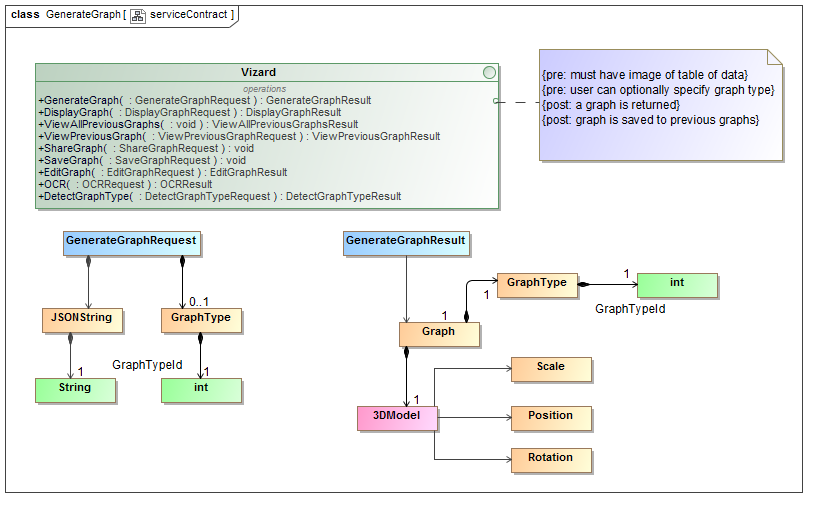
\includegraphics[width=\textwidth]{Images/class__GenerateGraph__serviceContract.png}  \\
		\caption{Services Contract : GenerateGraph}
	\end{figure}
	\begin{figure}[H]
		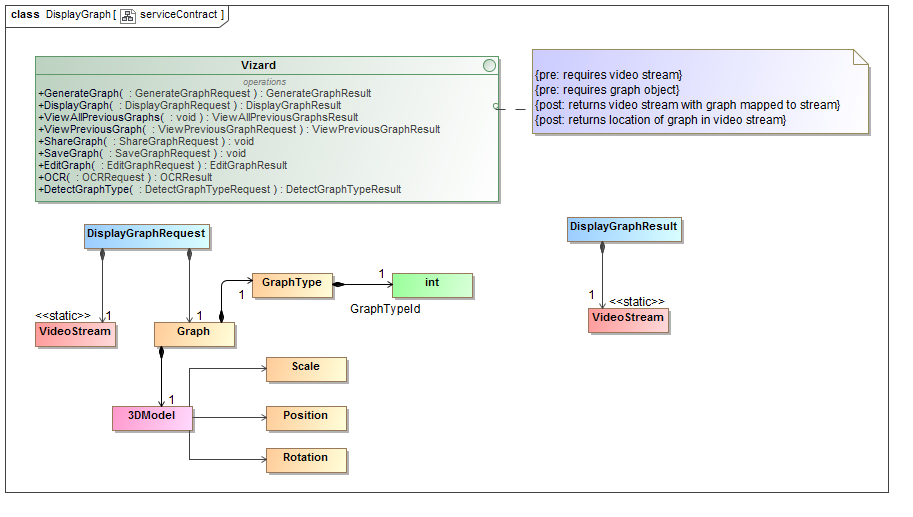
\includegraphics[width=\textwidth]{Images/class__DisplayGraph__serviceContract.png}  \\
		\caption{Services Contract : DisplayGraph}
	\end{figure}
	\begin{figure}[H]
		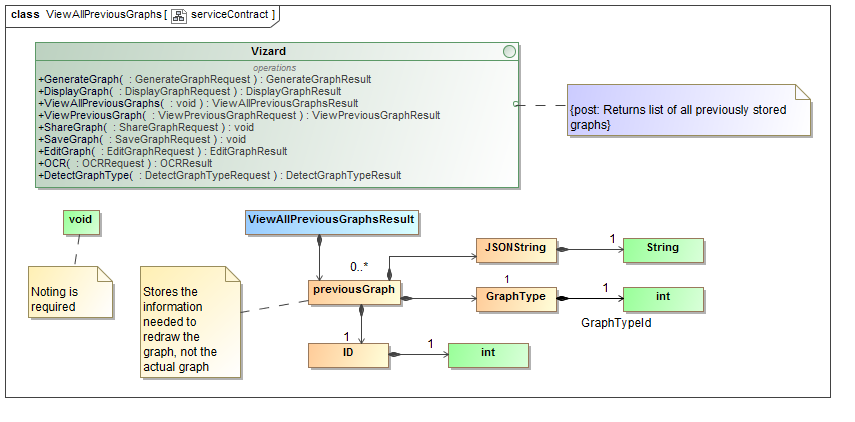
\includegraphics[width=\textwidth]{Images/class__ViewAllPreviousGraphs__serviceContract.png}  \\
		\caption{Services Contract : ViewAllPreviousGraphs}
	\end{figure}
	
	\begin{figure}[H]
		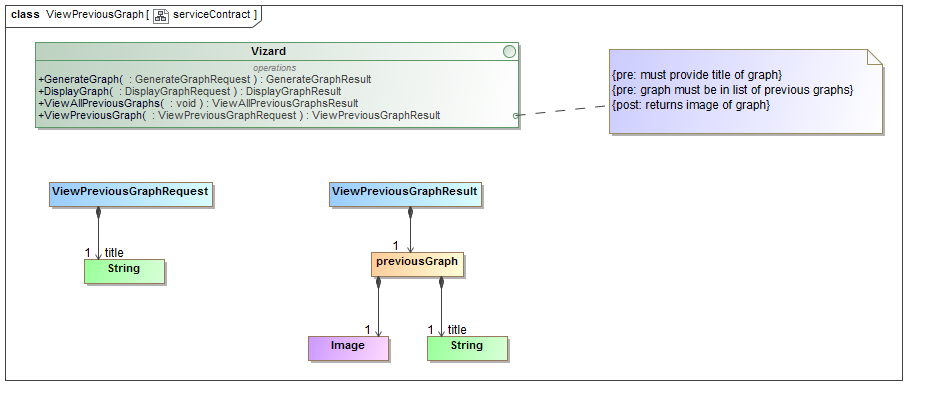
\includegraphics[width=\textwidth]{Images/class__ViewPreviousGraph__serviceContract.png}  \\
		\caption{Services Contract : ViewPreviousGraph}
	\end{figure}
	
	\begin{figure}[H]
		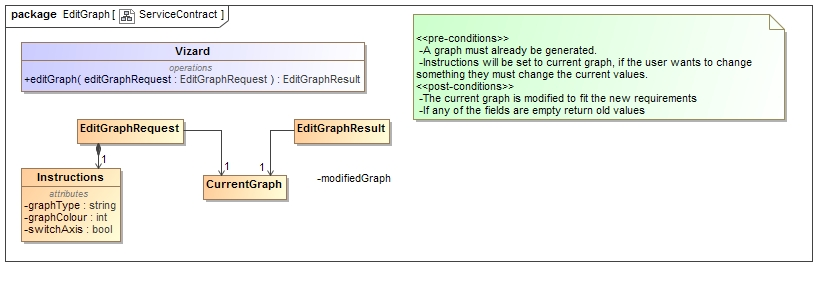
\includegraphics[width=\textwidth]{Images/class__EditGraph}  \\
		\caption{Services Contract : EditGraph}
	\end{figure}
	
	\begin{figure}[H]
		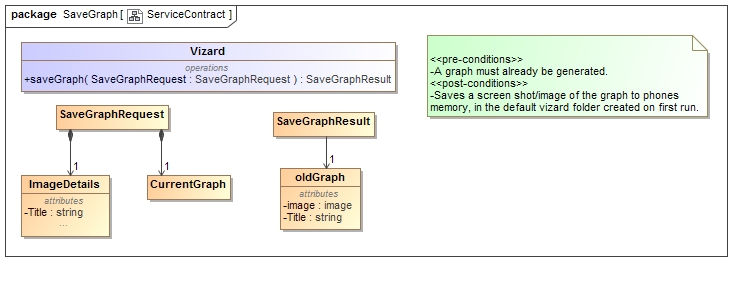
\includegraphics[width=\textwidth]{Images/class__SaveGraph}  \\
		\caption{Services Contract : SaveGraph}
	\end{figure}
	
	\begin{figure}[H]
		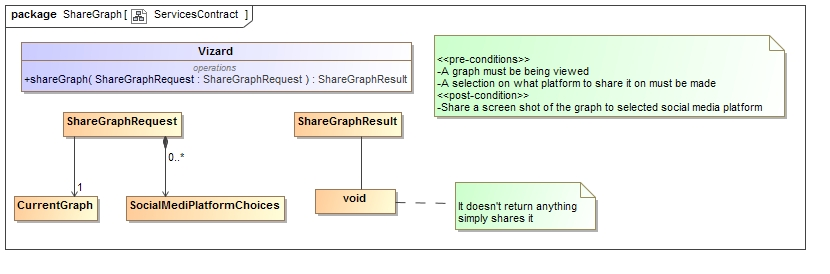
\includegraphics[width=\textwidth]{Images/class__ShareGraph}  \\
		\caption{Services Contract : ShareGraph}
	\end{figure}

\subsection{Required functionality}
	\begin{figure}[H]
		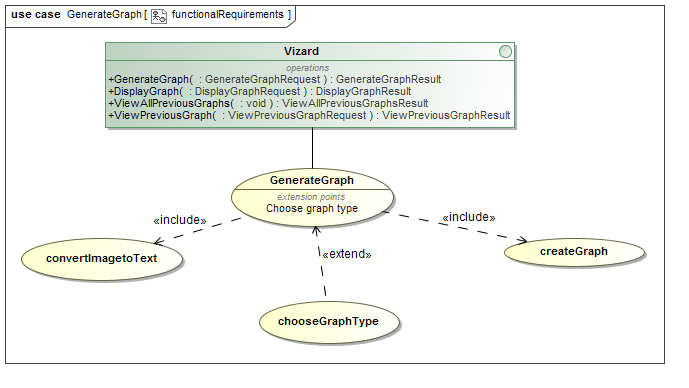
\includegraphics[width=\textwidth]{Images/uc__GenerateGraph__functionalRequirements.png}  \\
		\caption{Required functionality : GenerateGraph}
	\end{figure}
	\begin{figure}[H]
		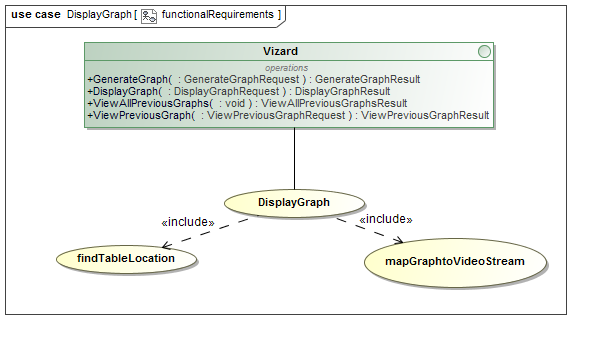
\includegraphics[width=\textwidth]{Images/uc__DisplayGraph__functionalRequirements.png}  \\
		\caption{Required functionality : DisplayGraph}
	\end{figure}
	\begin{figure}[H]
		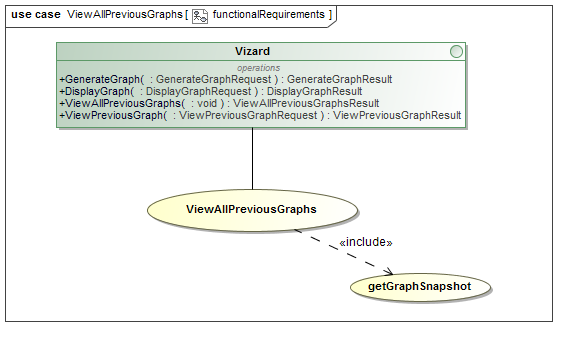
\includegraphics[width=\textwidth]{Images/uc__ViewAllPreviousGraphs__functionalRequirements.png}  \\
		\caption{Required functionality : ViewAllPreviousGraphs}
	\end{figure}
	\begin{figure}[H]
		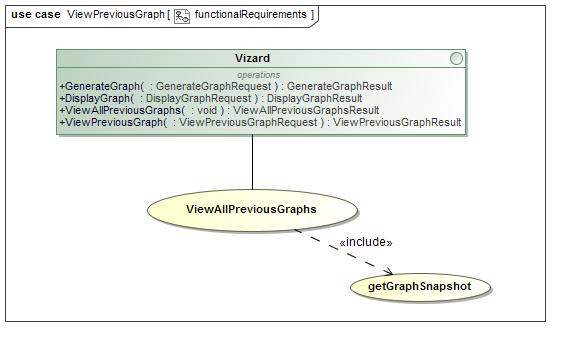
\includegraphics[width=\textwidth]{Images/uc__ViewPreviousGraph__functionalRequirements.png}  \\
		\caption{Required functionality : ViewPreviousGraph}
	\end{figure}	
	
	\begin{figure}[H]
		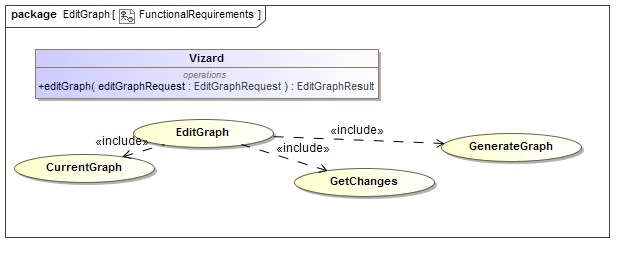
\includegraphics[width=\textwidth]{Images/uc__EditGraph}  \\
		\caption{Required functionality : EditGraph}
	\end{figure}
	
	\begin{figure}[H]
		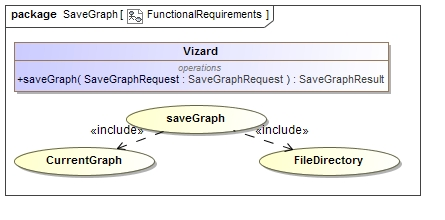
\includegraphics[width=\textwidth]{Images/uc__SaveGraph}  \\
		\caption{Required functionality : SaveGraph}
	\end{figure}
	
	\begin{figure}[H]
		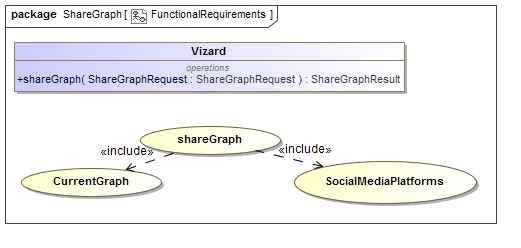
\includegraphics[width=\textwidth]{Images/uc__ShareGraph}  \\
		\caption{Required functionality : ShareGraph}
	\end{figure}

\subsection{Process specifications}
	\begin{figure}[H]
		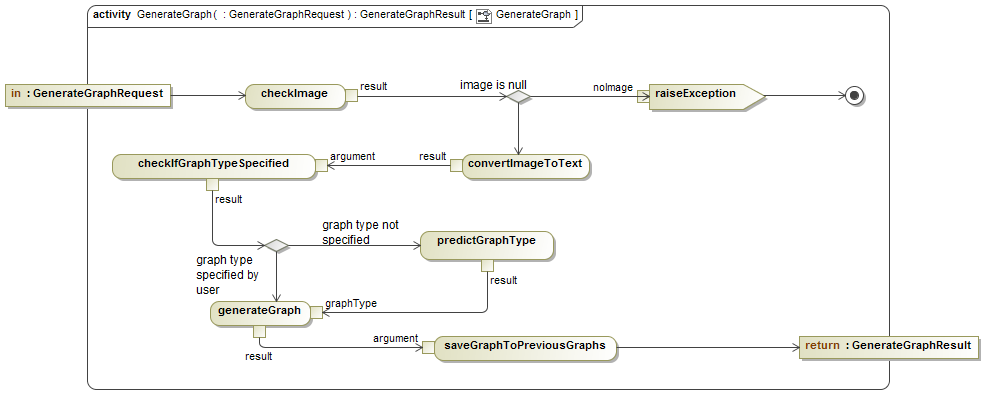
\includegraphics[width=\textwidth]{Images/act__GenerateGraph__GenerateGraph.png}  \\
		\caption{Process specifications : GenerateGraph}
	\end{figure}
	\begin{figure}[H]
		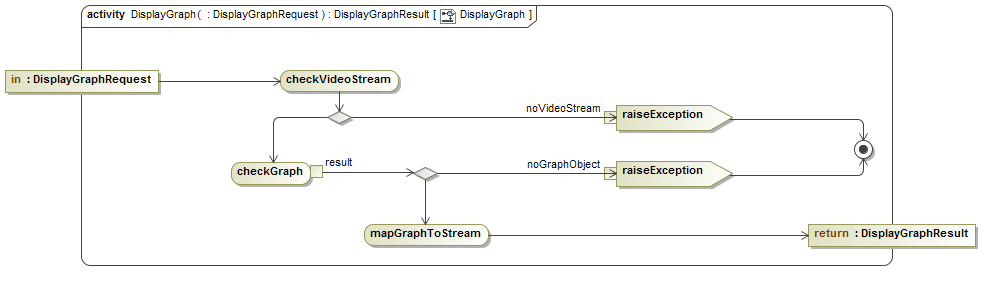
\includegraphics[width=\textwidth]{Images/act__DisplayGraph__DisplayGraph.png}  \\
		\caption{Process specifications : DisplayGraph}
	\end{figure}
	\begin{figure}[H]
		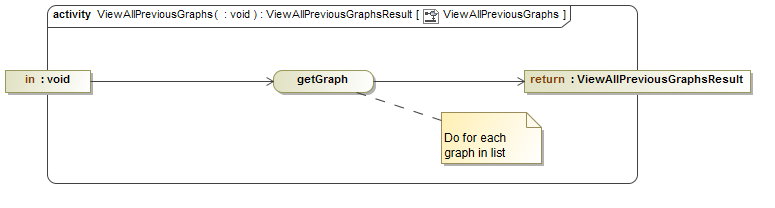
\includegraphics[width=\textwidth]{Images/act__ViewAllPreviousGraphs__ViewAllPreviousGraphs.png}  \\
		\caption{Process specifications : ViewAllPreviousGraphs}
	\end{figure}
	\begin{figure}[H]
		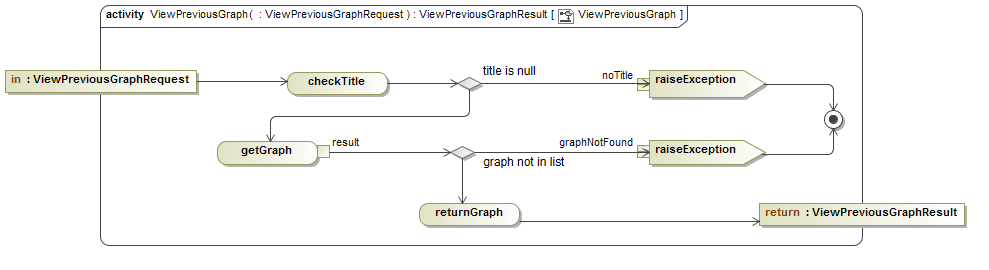
\includegraphics[width=\textwidth]{Images/act__ViewPreviousGraph__ViewPreviousGraph.png}  \\
		\caption{Process specifications : ViewPreviousGraph}
	\end{figure}
	
		\begin{figure}[H]
		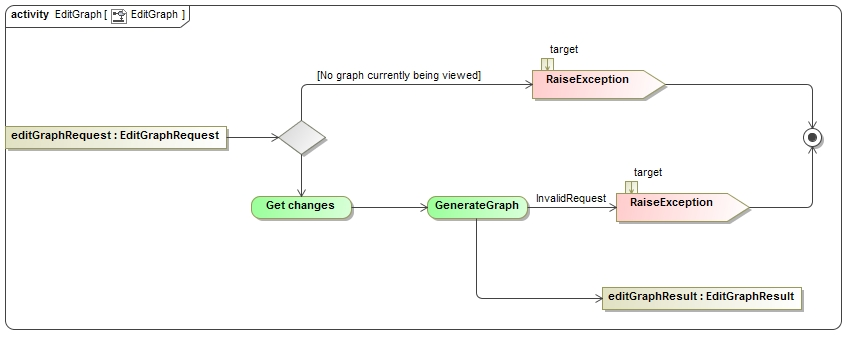
\includegraphics[width=\textwidth]{Images/act__EditGraph}  \\
		\caption{Process specifications : EditGraph}
	\end{figure}
	
	\begin{figure}[H]
		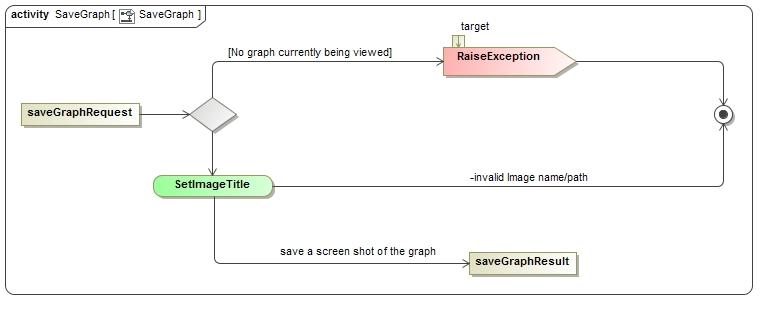
\includegraphics[width=\textwidth]{Images/act__SaveGraph}  \\
		\caption{Process specifications : SaveGraph}
	\end{figure}
	
	\begin{figure}[H]
		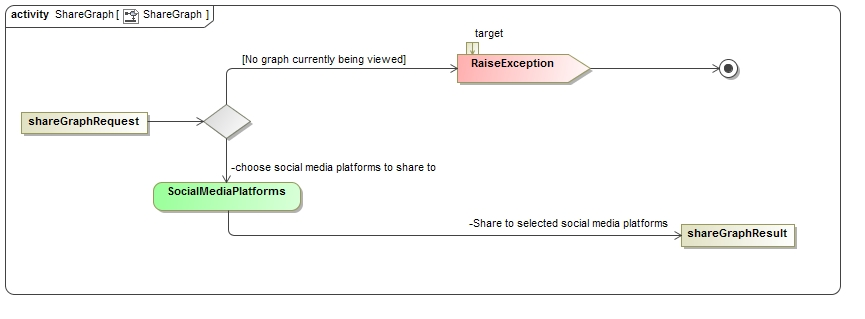
\includegraphics[width=\textwidth]{Images/act__ShareGraph}  \\
		\caption{Process specifications : ShareGraph}
	\end{figure}

%\subsection{Domain Model}

%\subsection{Use of Reference Architectures and Frameworks}

%\subsubsection{Web 2.0 Reference Architecture}

%\subsection{Access and Integration Channels}

\newpage
\section{Open Issues}


\end{document}
